Magnetized Liner Inertial Fusion (MagLIF) is an alternative approach to ICF fusion that takes advantage Z-pinch type confinement geometry. The MagLIF scheme sends intense currents axially up a cylindrical liner, generating a radial magnetic field which ultimately compresses the liner inward. This compression technology turns out to be significantly more efficient ($\sim10\%$) than laser approaches ($\sim1\%$) generally used in ICF schemes. The liner contains DT fuel, that get compressed with the liner and ideally ignites. In addition to this compression, an external axial magnetic field is applied to aid in the confinement of the fuel. In this way, MagLIF acts as a hybrid like approach between magnetic confinement and inertial confinement fusion. This is the major approach being explored at the Z Pulsed Power Facility discussed in Section \ref{sec:ZMachine}.

\begin{figure}[h!]
	\centering
	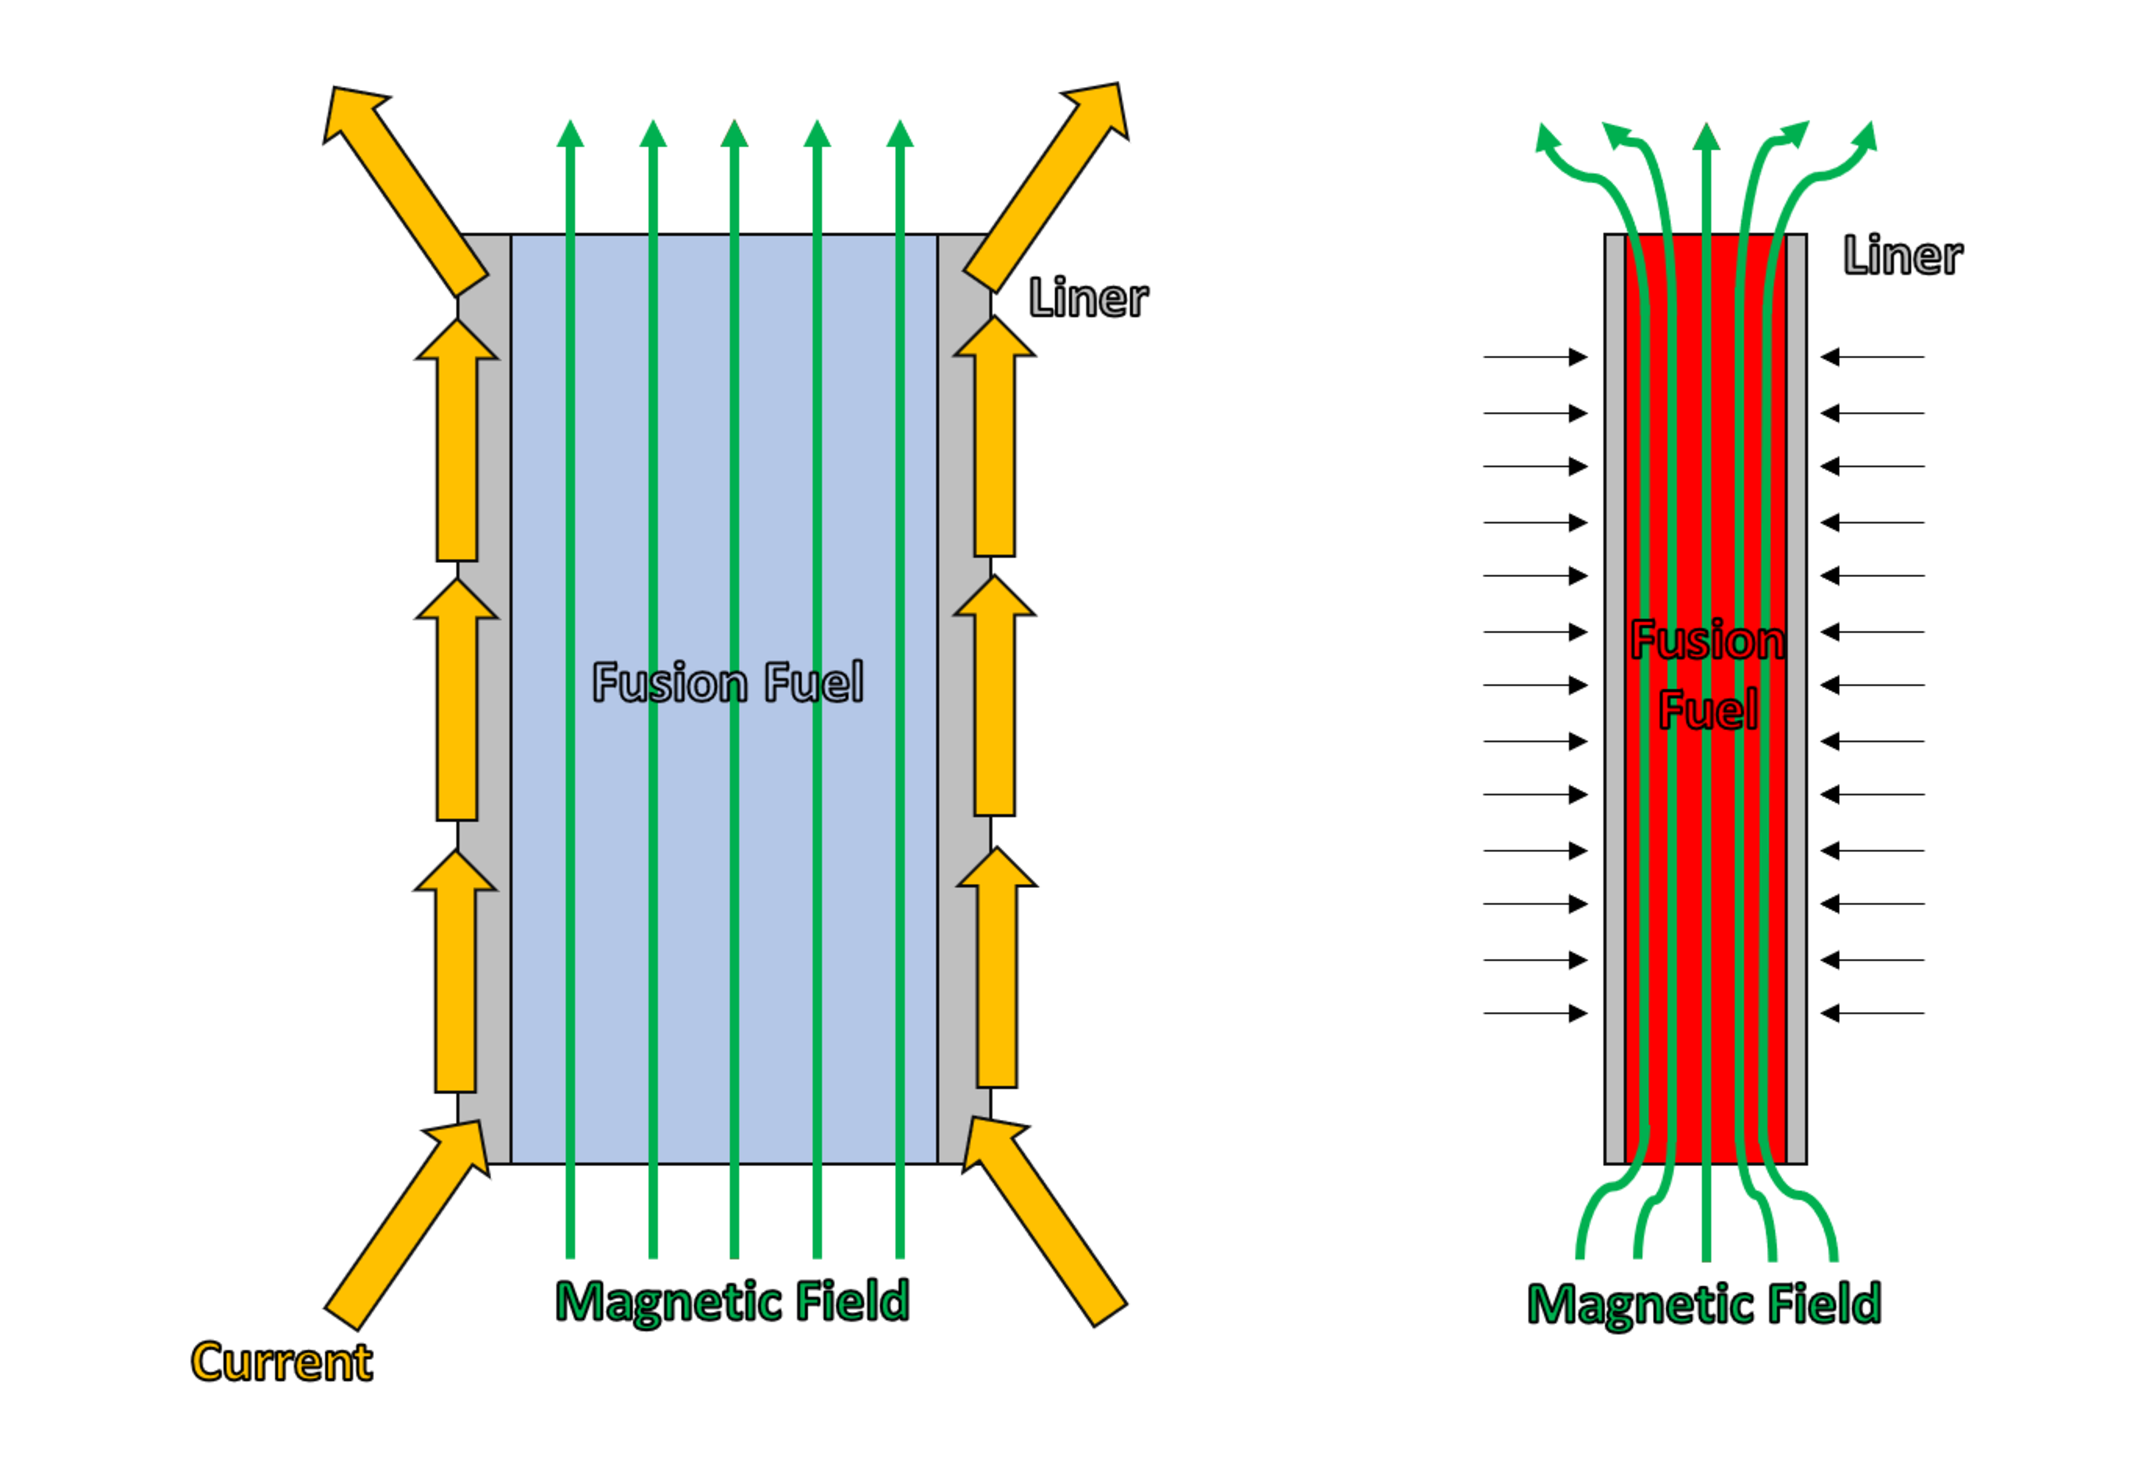
\includegraphics[scale=0.3]{Figures/magLIF.pdf}
	\caption{\todo{MAGLIF}}
	\label{fig:MagLIF}
\end{figure}

The unique nature of this approach changes the ignition requirements considerably. First off, the liner is designed to survive the compression meaning it provides a "cage" of the final burning fuel. This constricts the expansion for the burning plasma and significantly increases the confinement time. We can get an estimate of this confinement by using Newton's second law to describe the burning plasma pressing on a thin liner 
%
\begin{equation}
	M_l\frac{d^2R}{dt^2} = P_0(2\pi R)
\end{equation}
%
where $M_l$ is the mass per unit length of the liner, and $P_0$ is the pressure of the burning plasma. The characteristic time scale of this motion is the confinement time. It is given by:
%
\begin{equation}
	\tau \propto \sqrt{M_l / (2\pi P_0)}
\end{equation}
%
We can replace some of these values with terms that we are more familiar with:
%
\begin{equation}
	\tau \propto \frac{\sqrt{R}}{c_s}\sqrt{\frac{\rho_Lt_L}{\rho}}
\end{equation}
%
where $\rho_Lt_L$ is the areal density of the liner. Plugging this new confinement time into equation \ref{eq:burnFraction} gives us:
%
\begin{equation}
	\begin{split}
		f &= \frac{\sqrt{\rho R \rho_Lt_L}}{\sqrt{\rho R \rho_Lt_L} + H_B}
	\end{split}
\end{equation}
%
Here we've just assumed the same $1/4$ pre-factor as before for convenience. Note that the true burn fraction requires much more sophisticated simulations. Despite that though, this equation illustrates the advantage of the liner in reducing the required fuel areal density. Based on this scaling, a linear areal density of 5 mg/cm$^2$ reduces the required hot-spot areal density to 0.02 g/cm$^2$. This significantly reduces the required compression.

One disadvantage of this reduced areal density requirement is the confinement of the alpha particles. One happy coincidence of the ICF requirement of 0.3 g/cm$^2$ is that's approximately the range of a 3.5 MeV alpha particle. With only 0.02 g/cm$^2$, the alpha particles will freely stream into the liner without depositing their heat back into the hot-spot. The remedy for this is the external magnetic field. While this isn't the sole reason for the externally applied magnetic field, it does solve this problem by magnetically confining the alpha particles that travel radially. In order to accomplish this, the gyro radius of the alpha particles, must be of the order of the system radius:
%
\begin{equation}
	\begin{split}			
		R / R_\alpha &> 1 \\
		BR &> 26.5 \text{ Tesla-cm}
	\end{split}
\end{equation}
%
Here $R_\alpha$ is the gyro radius of a 3.5 MeV alpha particle, and $B$ is the axial magnetic field strength at peak compression. 

Of course, no such confinement exists axially so the areal density must be sufficiently large on axis. To ensure this we take:
%
\begin{equation}
	\rho H = 0.5 \text{ g/cm}^2
\end{equation}
%
where $H$ is the height of the liner.  

\todo{Due to constraints that are beyond the scope of this discussion, } this final hot-spot density needs to be of order 1 g/cm$^3$. This means we require a final radius of $R=200$ $\mu$m, a height of $H=1.0$ cm and a final magnetic field strength of over 1000 Tesla. This may seem unmanageable at first but the magnetic fields get compressed with the liner meaning our initial magnetic field strength can be much lower. A starting DT gas density of 5 mg/cc would imply convergences of the order of $15$ which correspond to an initial magnetic field strength as low as 6 Tesla. 

One last thing that should be noted is the fact that ignition temperatures cannot be reached by the slow cylindrical implosions that we have described. To get around this, MagLIF makes an additional alteration to the ICF scheme by preheating the fuel before it is compressed. This is done via a laser that penetrates the fuel from the top. See Figure \ref{fig:MagLIF} for a depiction of this.

\todo{Table comparing implosion parameters?}




